\chapter{Giới thiệu hệ thống}\label{chap1}
Trước khi đi sâu vào thiết kế kiến trúc của hệ thống quản lý quán ăn và các dịch vụ liên quan, chương này sẽ trình bày một số kiến thức cơ bản, quan trọng liên quan đến đề tài, các khái niệm, công nghệ sử dụng cho dự án.
Sau khi đã có một cái nhìn tổng quan, Mục \autoref{sec:main-functions} giới thiệu những nhiệm vụ chính của hệ thống theo thiết kế ban đầu và mối liên hệ giữa từng dịch vụ trong hệ thống đối với từng chức năng.

\section{Kiến trúc hệ thống}
% \subsection{Cây cú pháp trừu tượng và đồ thị dòng điều khiển} \label{sec:kno-ast-and-cfg}
Nền tảng hạ tầng của hệ thống được thiết kế giúp hướng đến tính ổn định cao và phát triển cho sau này.
Khi hệ thống đạt một số lượng người dùng nhất định, và có thể những người dùng này trải dài khắp nơi thay vì tập trung chủ yếu tại một địa điểm cố định.
Khi đó, việc duy trì một máy chủ vật lý sẽ không còn là lựa chọn tối ưu do sự tốn kém về nhân lực cũng như chi phí phát sinh trong việc bảo trì và nâng cấp cho máy chủ.
Từ đó mô hình kiến trúc của dự án hướng tới triển khai trên môi trường đám mây, tức sử dụng máy chủ của các nhà cung cấp dịch vụ đám mây rải rác ở khắp nơi trên thế giới.
Điều này sẽ giúp giảm đáng kể thời gian cấu hình máy chủ vật lý của hệ thống cũng như thời gian cần phải bỏ ra giúp duy trì và bảo dưỡng do các tác nhân bên ngoài gây nên.

Hình \ref{fig:overall-architecture} dưới đây mô tả kiến trúc tổng quan của nền tảng quản lý quán ăn triển khai trên môi trường đám mây.

\begin{figure}[h]
	\centering
	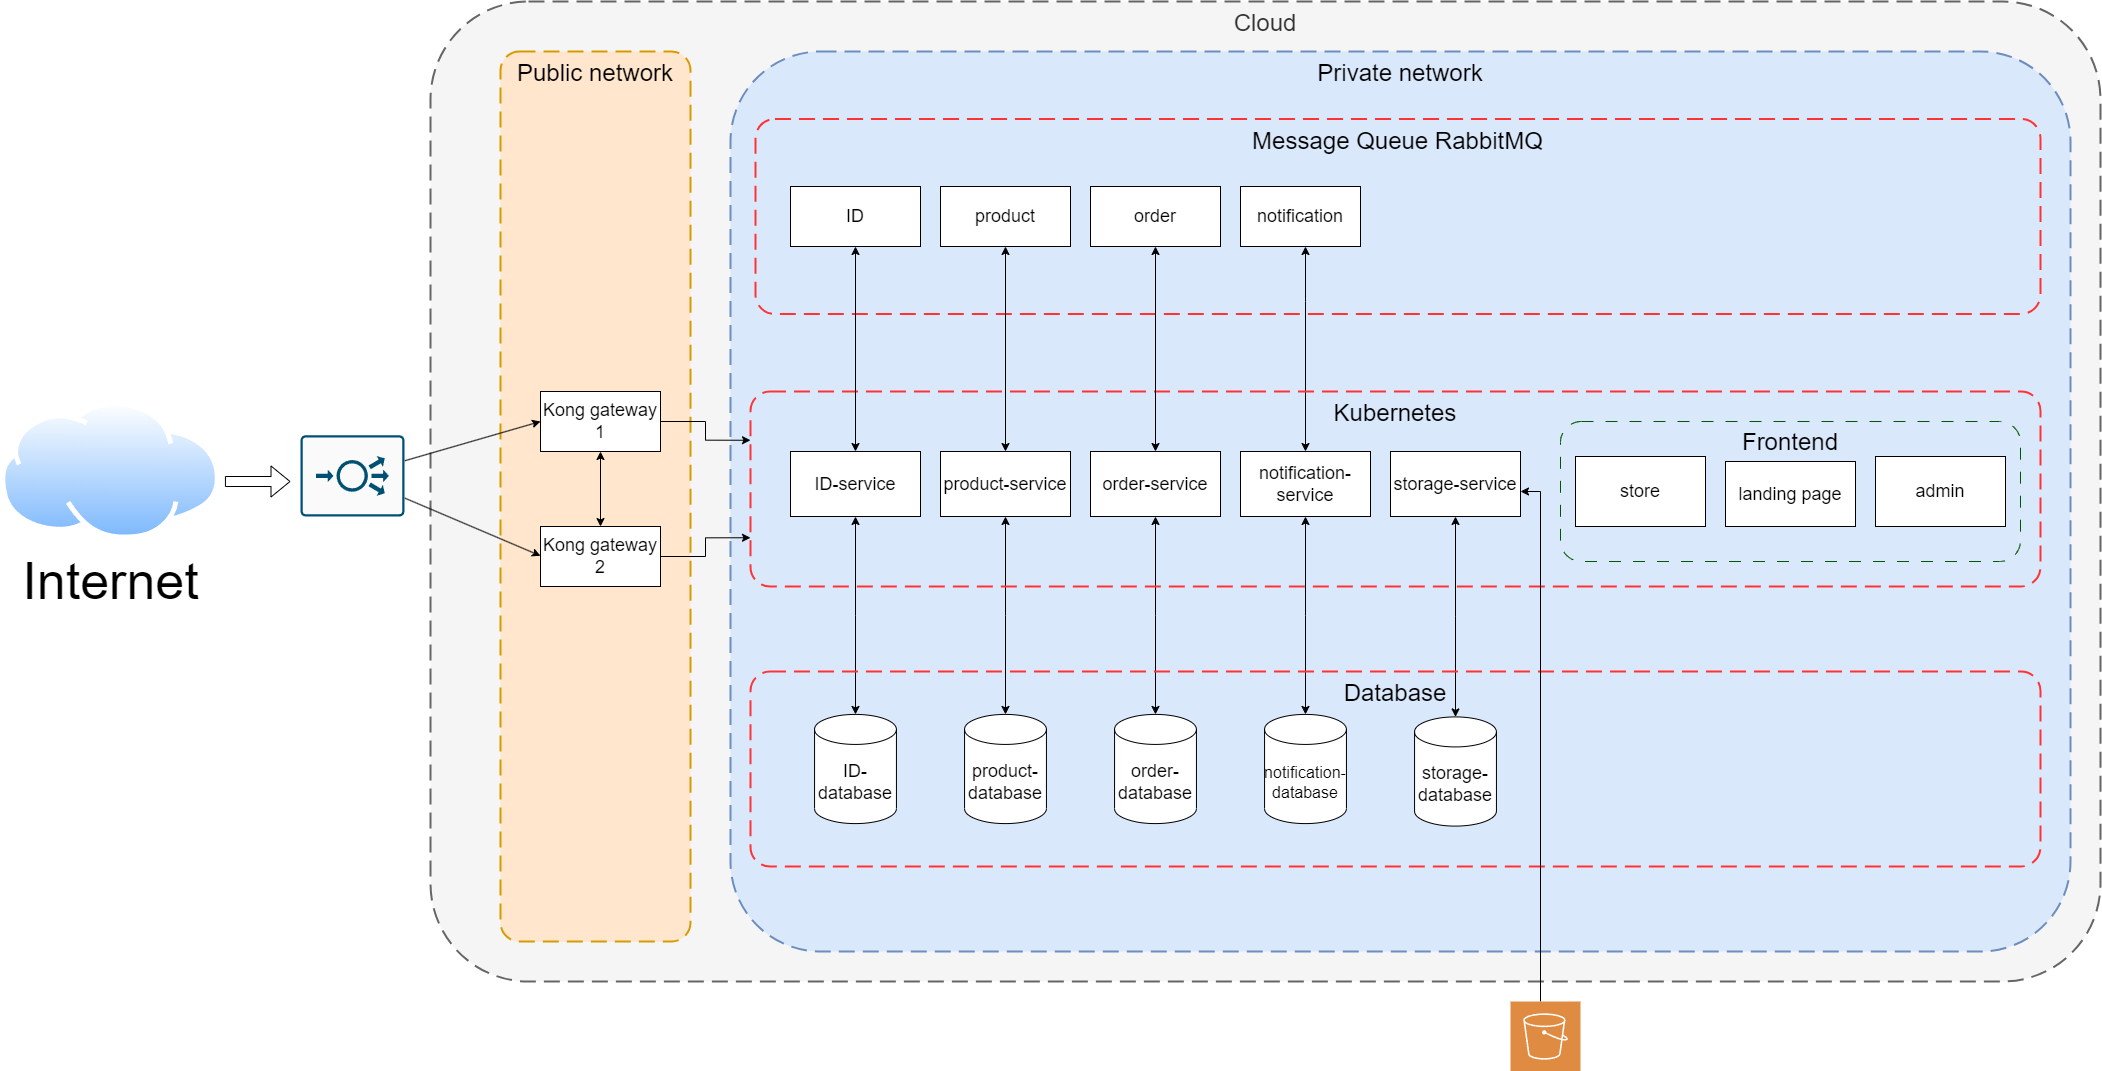
\includegraphics[width=1.1\textwidth]{images/hChip/overall-architecture.png}
	\caption{Hình vẽ mô tả kiến trúc tổng quan của hệ thống quản lý quán ăn}
	\label{fig:overall-architecture}
\end{figure}

Luồng dữ liệu đi vào hệ thống bắt nguồn từ ngoài Internet, nơi tất cả các yêu cầu của người dùng đi qua một GLSB (Global Server Load Balancers).
Ở đây GSLB của hệ thống được triển khai trên Cloudflare giúp phân phối người dùng ở bất cứ nơi nào trên thế giới đến máy chủ khỏe mạnh gần nhất đối với họ.
Điều này sẽ giúp tối ưu hóa thời gian tải trang, giảm thiểu độ trễ, và đảm bảo trải nghiệm truy cập website của người dùng nhanh chóng, mượt mà nhất.

Ngoài ra Cloudflare còn đóng vai trò như một hệ thống phân giải tên miền (DNS).
Khi người dùng truy cập vào trang của hệ thống lần đầu tiên trên trình duyệt web, trình duyệt sẽ gửi truy vấn tới máy chủ DNS cục bộ (resolver), thông thường sẽ là máy chủ của nhà mạng.
Máy chủ DNS cục bộ sẽ kiểm tra liệu tên miền đang được yêu cầu có địa chỉ IP tương ứng không, nếu không tìm thấy máy chủ DNS của nhà mạng sẽ thực hiện một lời gọi khác tới máy chủ DNS tại các cấp cao hơn.
Ở đây cấp độ ngay trên máy chủ cục bộ của nhà mạng sẽ là các máy chủ DNS nơi máy chủ được triển khai như Cloudflare hoặc Google Cloud.
Lời gọi sẽ được chuyển đến DNS của nhà cung cấp mạng của người dùng và sau đó là đến Cloudflare DNS.
Cloudflare sẽ nhận lời gọi của người dùng với tên miền của hệ thống đã được đăng ký trên Namecheap\footnote{https://www.namecheap.com/} và người dùng đến địa chỉ IP (Internet Protocol) của máy chủ phù hợp nhất với người gọi.

Bên trong mỗi máy chủ được triển khai trên Google Cloud sẽ có hai lớp mạng là mạng công cộng được phơi ra ngoài Internet và lớp mạng nội bộ nơi triển khai các thành phần chức năng chính.
Tại lớp mạng công cộng triển khai hai cổng API (API Gateway) phụ trợ cho nhau.
Ngoài những lợi ích chính của một cổng API đó là giúp thống nhất một điểm truy cập đến máy chủ thông qua API Gateway và cải thiện hiệu suất hệ thống nhờ cơ chế cache kết quả truy vấn API cũng như là giới hạn lưu lượng truy cập tránh quá tải, việc sử dụng song song hai cổng API cũng giúp phân phối lưu lượng truy cập giữa các cổng và giúp đảm bảo tính sẵn sàng cao cho hệ thống.

Các cổng API sau đó sẽ chuyển tiếp lời gọi từ ngoài Internet đến hệ thống mạng nội bộ của máy chủ, nơi sẽ triển khai các thành phần chính của mô hình quản lý quán ăn.
Hệ thống ở đây được chia thành ba lớp chính bao gồm lớp hàng đợi tin nhắn sử dụng RabbitMQ, lớp K8s bao gồm các dịch vụ phụ trách xử lý lời gọi của người dùng, và cuối cùng là lớp cơ sở dữ liệu lưu trữ các thông tin quan trọng như dữ liệu của người dùng, nhà hàng, quán ăn, v.v..
Hệ thống được thiết kế theo hướng kiến trúc vi dịch vụ (microservice) tức từng thành phần, chức năng chính của hệ thống sẽ được triển khai và hoạt động trên các môi trường độc lập với nhau giúp hệ thống chịu lỗi tốt hơn, bảo trì dễ dàng, và tiện lợi trong việc nâng cấp, mở rộng sau này.
Mỗi vi dịch vụ microservice có trách nhiệm thực hiện một chức năng cụ thể, ví dụ như dịch vụ thông báo sẽ hoạt động với mục đích duy nhất là nhận thông tin được đẩy đến từ một hoặc nhiều dịch vụ cụ thể và phân phối nó đến với các dịch vụ đã đăng ký nhận thông báo từ các dịch vụ đó.
Việc chia nhỏ hệ thống thành các dịch vụ độc lập mang lại nhiều lợi ích như giúp dễ dàng triển khai và bảo trì cho hệ thống, tăng tính sẵn sàng cũng như là khả năng chịu lỗi, giúp tự động mở rộng hệ thống.
Về mặt phát triển hệ thống, bởi vì mỗi vi dịch vụ đều hoàn toàn độc lập với nhau nên các đội ngũ phát triển của từng chức năng có thể chọn bộ công nghệ phù hợp nhất với nhu cầu và khả năng của đội.

Nền tảng quản lý quán ăn trên hình \ref{fig:overall-architecture} được triển khai nền tảng Kubernetes (K8s) và Google Cloud Platform (GCP) mang đến nhiều lợi ích cho việc vận hành và quản lý ứng dụng.
K8s là một nền tảng mã nguồn mở giúp tự động hóa việc triển khai, quản lý và mở rộng các ứng dụng đóng gói\footnote{https://kubernetes.io/docs/concepts/overview/}.
Sử dụng K8s cho hệ thống vi dịch vụ (microservice) giúp giảm tải đáng kể công sức triển khai từng dịch vụ độc lập một cũng như mở rộng, quản lý các dịch vụ này do K8s có thể được cấu hình để tự động hóa các tác vụ thủ công như tạo và quản lý các Docker container, tự động phục hồi và xử lý lỗi.
Các ưu điểm công nghệ của K8s sẽ được đề cập rõ hơn trong Chương \textcolor{red}{Trích dẫn đến phần chi tiết triển khai hệ thống khi cấu hình K8s cho từng pod}
GCP cung cấp một nền tảng đám mây với gói chức năng đa dạng kèm theo các công cụ hỗ trợ tốt cho hệ thống với kiến trúc vi dịch vụ (microservice) giúp dễ dàng triển khai và vận hành.
Có thể kể đến nền tảng GKE giúp người dùng cấu hình K8s trên GCP một cách dễ dàng, Firebase giúp bảo mật hệ thống, xác thực người dùng truy cập vào hệ thống thông qua việc tạo lập và quản lý tài khoản cả người dùng.
GCP cũng hỗ trợ người sử dụng tránh được các vấn đề liên quan đến cấu hình cơ sở hạ tầng của hệ thống.
Với các tùy chọn đa dạng, người dùng có thể dựa theo nhu cầu thực tế của hệ thống tại từng thời điểm và chọn cấu hình phù hợp.

Tất cả thông tin của người dùng cũng như là nhà hàng, quán ăn tham gia vào nền tảng đều sẽ được lưu trong cơ sở dữ liệu của hệ thống. Các thông tin này có thể là về những lần đặt bàn, thực đơn của quán ăn, những lần gọi món của người dùng, thông tin người dùng, v.v., hoặc thông tin của hệ thống như các chỉ số sức khỏe, các bản ghi hoạt động, v.v.. Nền tảng quản lý quán ăn của khóa luận hiện tại sử dụng MongoDB\footnote{https://www.mongodb.com/}, một cơ sở dữ liệu dạng NoSQL. Chi tiết về cơ sở dữ liệu sẽ được nói rõ hơn trong Mục \autoref{sec:tehcnologies-used}.

\section{Các chức năng chính}\label{sec:main-functions}
Mô hình quản lý quán ăn được phát triển trong khóa luận này sẽ tập trung vào các chức năng chính giúp nhà hàng, quán ăn quản lý thực đơn, khách và bàn, v.v..
Từ các chức năng chính như quản lý thực đơn sẽ có các chức năng nhỏ hơn bổ trợ cho chức năng chính.
Ví dụ như đối với chức năng quản lý bàn, ngoài các chức năng chính như tạo bàn mới, xóa bàn, thay đổi trạng thái của bàn, v.v., các nhánh chức năng phụ còn bao gồm các chức năng như ghép bàn, gán bàn cho những người đặt bàn trước, v.v..
Điều này giúp cho 

Hình \textcolor{red}{Vẽ UML từ Copy of hChip trên Miro và chuyển vào đây} mô tả các chức năng chính của mô hình quản lý quán ăn.


\section{Luồng nghiệp vụ} \label{sec:handle-undef}
Pha xử lý hàm thiếu định nghĩa được bổ sung với hai nhiệm vụ chính đó là xử lý nguyên mẫu hàm cơ bản thiếu định nghĩa tìm được bởi trình biên dịch và xử lý nguyên mẫu hàm ảo thiếu định nghĩa mà trình biên dịch không thể phát hiện được. Ý tưởng chung để giải quyết hai nhiệm vụ vừa đề cập dựa trên việc tìm kiếm các ứng viên nguyên mẫu hàm tương thích trong mã nguồn kiểm thử theo các tiêu chí thích hợp, sau đó sinh thân hàm giả cho các ứng viên này. Mục \autoref{sec:handle-undef-first} mô tả cụ thể về phương pháp xử lý nhiệm vụ thứ nhất. Phương pháp xử lý nguyên mẫu hàm ảo được trình bày trong Mục \autoref{sec:handle-undef-second}.

% \subsection{Xử lý nguyên mẫu hàm cơ bản thiếu định nghĩa tìm bởi trình biên dịch} \label{sec:handle-undef-first}
Khóa luận đề xuất phương pháp sử dụng trình biên dịch để tìm kiếm các nguyên mẫu hàm cần sinh thân hàm giả trong mã nguồn kiểm thử. Thuật toán \autoref{alg:handle-ref} mô tả chi tiết quá trình tìm kiếm và xử lý các nguyên mẫu hàm cơ bản thiếu định nghĩa. Trước hết, thuật toán bắt đầu bằng việc thu thập danh sách các nguyên mẫu hàm cơ bản cần quan tâm trong tập các tệp mã nguồn $S$ và khởi tạo tập $T$ rỗng. Danh sách trả về bao gồm các xâu ký tự, mỗi xâu biểu thị một hàm bao gồm tên hàm và danh sách tham số của hàm đó (dòng~1-2). Tập $T$ là tập hợp các nguyên mẫu hàm trong mã nguồn kiểm thử được sinh thân hàm giả. Sau khi có danh sách, thuật toán xử lý từng xâu trong danh sách đầu vào (dòng~3-14). Cụ thể, với mỗi xâu, một AST $undef\_ast$ được xây dựng từ chữ ký hàm mà xâu biểu thị (dòng~4). Tiếp đó, tên của nguyên mẫu hàm được trích xuất từ AST vừa xây dựng (dòng~5) và tập các nguyên mẫu hàm ứng viên có cùng tên trong mã nguồn kiểm thử được thu thập và lưu vào danh sách $candidates$ (dòng~6). Danh sách tham số của nguyên mẫu hàm $undef$ và phạm vi định danh (scope qualifier) được trích xuất từ AST phục vụ cho quá trình lọc (dòng~7-8). Danh sách ứng viên được lọc bởi Thuật toán~\ref{alg:filter-undef} và thu được các ứng viên hợp lệ $qualified\_cans$ (dòng~9). Cuối cùng, từng ứng viên hợp lệ $qc$ được sinh thân hàm giả và thêm vào tập $T$ (dòng~11-12). Dữ liệu trong tập $T$ được lưu lại để xây dựng môi trường kiểm thử cho mã nguồn đang xét trong các lần sau mà không cần xử lý lại từ đầu.

\begin{algorithm}[ht]
    \small
    \caption{Thuật toán xử lý hàm thiếu định nghĩa}
    \label{alg:handle-ref}
    \SetKwComment{Comment}{/* }{ */} 
    \KwIn{~$S$ - collection of source code files}
    \KwOut{~$T$ - collection of handled undefined functions}
					
    $undefined\_functions \leftarrow $ Get necessary undefined functions in $S$\;
    $T \leftarrow \emptyset$\;
    \For {$undef : undefined\_functions$} {
        $undef\_ast\leftarrow$ Construct AST from the string $undef$\;
        $undef\_name \leftarrow$ Get the name of the function from string $undef\_ast$\;
        $candidates \leftarrow$ Find all function prototypes having the same name with $undef\_name$ in source code\;
        $undef\_params \leftarrow$ Extract a list of parameters from $undef\_ast$\;
        $undef\_scope\leftarrow$ Extract function scope qualifier from $undef\_ast$\;
        $qualified\_cans\leftarrow$ \textbf{call} Algorithm \autoref{alg:filter-undef} $(undef\_params, undef\_scope, candidates)$\;
        \For {$qc : qualified\_cans$} {
            $t \leftarrow $ Generate simple function body for $qc$\;
            $T \leftarrow T \cup {t}$
        }
    }

    \Return $T$
\end{algorithm}

% \subsubsection*{Thu thập danh sách nguyên mẫu hàm cơ bản thiếu định nghĩa}\label{sec:find-undef}
Ý tưởng sử dụng các công cụ tiện ích của trình biên dịch để tìm nguyên mẫu hàm cần quan tâm xuất phát từ lợi thế trình biên dịch biết hàm nào sẽ được sử dụng trong các tệp đối tượng như đã trình bày ở Mục \autoref{sec:kno-undefine}. Đoạn mã \autoref{cod:command-undef} mô tả cách dùng các công cụ tiện ích có trong trình biên dịch để tìm các nguyên mẫu hàm thiếu định nghĩa. Đầu tiên, phương pháp đề xuất sử dụng công cụ \textit{g++} với cờ \textit{-c} để biên dịch các tệp mã nguồn thành tệp đối tượng (object file) có đuôi \textit{.o} (dòng 1). Sau đó, các tệp đối tượng này sẽ được liên kết bởi công cụ liên kết \textit{ld} và cờ \textit{-r} thành một tệp đối tượng tổng hợp \textit{temp.o} (dòng 2). Lí do phương pháp đề xuất sử dụng công cụ liên kết \textit{ld} thay vì \textit{g++} là bởi \textit{g++} yêu cầu người dùng phải hoàn thiện tất cả các nguyên mẫu hàm bị thiếu định nghĩa trước khi liên kết thành tệp tổng hợp. Cuối cùng, tệp đối tượng tổng hợp được phân tích bởi công cụ phân tích ký hiệu \textit{nm}\footnote{https://sourceware.org/binutils/docs/binutils/nm.html} với các cờ \textit{-u} - trích xuất các hàm thiếu định nghĩa, \textit{-C} - chuyển ký hiệu máy thành ngôn ngữ lập trình C++ (dòng 3). Đầu ra của công cụ \textit{nm} sẽ được ghi vào tệp \textit{list.txt}.\\

\begin{lstlisting}[language=C++, caption={Các câu lệnh tìm nguyên mẫu hàm thiếu định nghĩa cần quan tâm sử dụng trình biên dịch.}, label={cod:command-undef},  captionpos=b]
g++ -c *.cpp
ld -r *.o -o temp.o
nm temp.o -u -C > list.txt
\end{lstlisting}

\begin{figure}[t]
    \begin{minipage}[t]{0.49\linewidth}
    \begin{lstlisting}[language=C++, caption={Mã nguồn tệp a.cpp.}, label={cod:undef-cpp}, captionpos=b]
// a.cpp
#include "a.hpp"
#include "b.hpp"
    
int foo(A *a, int x) {
    int ret = a->bar(true);
    int max = maxT<int>(x, ret);
    max += a->echo();
    const int *p = &(a->x);
    ret -= func(p, max);
    return ret;
}

void gamma(A *a, int x) {
    double max = maxT<double>(x, a->x);
    a->x = max;
}
int unused(int x);
    \end{lstlisting}
    \end{minipage}
    \begin{minipage}[t]{0.49\linewidth}
    \begin{lstlisting}[language=C++, caption={Mã nguồn tệp a.hpp, b.hpp và c.hpp.}, label={cod:undef-hpp}, captionpos=b]
// a.hpp
#include "c.hpp"
class A {
public: 
    int x;
    A(int _x) { x = _x; }
    int bar(bool b);
    double echo() {
        return x + delta(&x);
    }
};
int bar(bool b);
// b.hpp
template <typename T> T max(T a);
int func(int *a, int b);
int func(const int* a, int b);
    
// c.hpp
double delta(int* const x);  
    \end{lstlisting}
\end{minipage}
\end{figure}

Các Đoạn mã \autoref{cod:undef-cpp}, \autoref{cod:undef-hpp} minh họa cách áp dụng phương pháp đề xuất trên tập đơn vị kiểm thử cần xử lý các nguyên mẫu hàm cơ bản thiếu định nghĩa với bốn tệp mã nguồn. Kiểm thử viên muốn kiểm thử tự động cho hai hàm có logic đầy đủ \tcode{foo} và \tcode{gamma}. Hai hàm này chứa mã nguồn đầy đủ. Hai đoạn mã chứa một số nguyên mẫu hàm đó là \tcode{unused}, \tcode{bar}, \tcode{delta} và ba hàm trong tệp \tcode{b.hpp}. Hàm \tcode{foo} trong Đoạn mã \autoref{cod:undef-cpp} nhận đầu vào là một biến con trỏ đến đối tượng của lớp \tcode{A} và một biến kiểu nguyên \tcode{x}. Logic mã nguồn của \tcode{foo} gọi tới hai phương thức của biến \tcode{a} đó là \tcode{bar} và \tcode{echo}. Ngoài ra, hàm \tcode{foo} còn gọi tới nguyên mẫu hàm template \tcode{maxT} với kiểu khởi tạo \tcode{int} và hàm \tcode{func(const int* a, int b)} thuộc tệp \tcode{b.hpp}. Hàm \tcode{gamma} cũng có các đầu vào tương tự nhưng gọi nguyên mẫu hàm \tcode{maxT} nhưng sử dụng tham số kiểu \tcode{double} thay vì \tcode{int} như hàm \tcode{foo}.
\vspace{5mm}
\begin{figure}[h]
	\begin{lstlisting}[language=C++, caption={Danh sách các nguyên mẫu hàm thiếu định nghĩa tìm bởi trình biên dịch.}, label={cod:result-undef}, captionpos=b]
func(int const*, int)
double maxT<double>(double, double)        
int maxT<int>(int, int)     
delta(int*)
A::bar(bool)         
	\end{lstlisting}
\end{figure}

Đoạn mã \autoref{cod:result-undef} minh họa danh sách các nguyên mẫu hàm cần quan tâm trong tệp các đơn vị kiểm thử \textit{a.cpp}, \textit{a.hpp}, \textit{b.hpp} và \textit{c.hpp} khi áp dụng phương pháp đề xuất. Dòng đầu tiên cho biết nguyên mẫu hàm \tcode{func(int const*, int)} cần được xử lý, tương đương với hàm \tcode{func(const int* a, int b)} trong mã nguồn \textit{b.hpp} (dòng 16 trong Đoạn~mã~\autoref{cod:undef-hpp}). Dòng 2 và 3 biểu thị cú pháp của hàm template. Đối với trình biên dịch, các lời gọi hàm template với các kiểu đối số khác nhau sẽ tạo ra các chữ ký hàm khác nhau. Do hàm \tcode{foo} và \tcode{gamma} gọi hàm \tcode{maxT} với hai đối số kiểu khác nhau nên danh sách các nguyên mẫu hàm thiếu định nghĩa chứa chữ ký hàm cho cả hai kiểu này. Tiếp theo, nguyên mẫu hàm ở dòng 4 tương ứng hàm \tcode{delta(int* const x)} trong tệp c.hpp. Tham số hiển thị ở tệp mã nguồn và trên danh sách khác nhau là bởi trình biên dịch chỉ quan tâm tới kiểu của tham số và loại bỏ lớp lưu trữ (storage class) ngoài cùng của tham số đó. Tham số \tcode{x} của hàm \tcode{delta} có kiểu là \tcode{int* const} tức con trỏ hằng trỏ tới một biến kiểu nguyên. Trình biên dịch chuyển kiểu của tham số trên thành \tcode{int*}. Trong trường hợp của hai hàm \tcode{func}, tham số đầu của hai hàm khác nhau là bởi tham số \tcode{const int* a} được trình biên dịch chuyển thành kiểu \tcode{const int*} do từ khoá \tcode{const} là lớp lưu trữ của biến được tham số trỏ tới. Cuối cùng nguyên mẫu hàm \tcode{A::bar(bool)} tương ứng với nguyên mẫu hàm \tcode{int bar(bool b)} trong lớp \tcode{A} (dòng 7 trong Đoạn mã \autoref{cod:undef-hpp}).

% \subsubsection*{Lọc tìm ứng viên hợp lệ}
Như đã mô tả trong ví dụ minh hoạ ở Đoạn mã \autoref{cod:result-undef}, mỗi nguyên mẫu hàm trong danh sách trả về bởi trình biên dịch sẽ tương ứng với một số nguyên mẫu hàm cơ bản trong mã nguồn gốc. Để ánh xạ từng nguyên mẫu hàm cần quan tâm tới đúng nguyên mẫu hàm cơ bản trong đơn vị kiểm thử, phương pháp đề xuất sử dụng ba tiêu chí để đánh giá độ phù hợp của từng ứng viên. Tiêu chí đầu tiên đó là hàm ứng viên chưa được ánh xạ bởi bất kỳ nguyên mẫu hàm nào trên danh sách. Tiêu chí thứ hai đó là số lượng tham số và phạm vi định danh của hai hàm phải giống nhau. Tiêu chí này giúp giảm số lượng các ứng viên có cùng tên cần xét. Cuối cùng, ứng viên hợp lệ nếu từng tham số đã chuẩn hoá của ứng viên có cùng kiểu với tham số tương ứng của nguyên mẫu hàm.
\begin{algorithm}
    \small
    \caption{Thuật toán lọc tìm ứng viên hợp lệ}
    \label{alg:filter-undef}
    \SetKwComment{Comment}{/* }{ */} 
    \KwIn{~$undef\_params$ - list of parameters extracted from the string $undef$ \\
    \hskip 1.1cm $undef\_scope$ - the scope qualifier of $undef$\\
    \hskip 1.1cm  $candidates$ - list of function prototypes having the same name
    }
    \KwOut{~$qualified\_cans$ - list of qualified function prototypes}
					
    $qualified\_cans \leftarrow$ Initial empty list\;
    \For {$candidate : candidates$} {
        \uIf {$candidate$ \textbf{is} \textit{handled}} {
            \textbf{continue}
        }
        \Else {
            $can\_params \leftarrow$ Extract a list of parameters of function $candidate$\;
            $can\_scope\leftarrow$ Get the scope qualifier of $candidate$\;
            \uIf {$can\_params.length \neq undef\_params.length$ \textbf{or} $can\_scope \neq undef\_scope$} {
                \textbf{continue}
            }
            \Else {
                $same\_params \leftarrow$ \textbf{True}\;
                $iter\leftarrow$ 1 \Comment*[r]{Assume the list starts at index 1}
                \While{$iter \leq can\_params.length$} {
                    $can\_param\_iter\leftarrow$ Normalize the $iter^{th}$ param of $can\_params$\;
                    $undef\_param\leftarrow$ Get the $iter^{th}$ param of $under\_params$ \;
                    \uIf{$can\_param\_iter$ \textbf{has the same type with} $under\_params$} {
                        $iter++$
                    }
                    \Else {
                        $same\_params\leftarrow$ \textbf{False}\;
                        \textbf{break}
                    }
                }

                \If{$same\_params\leftarrow$ \textbf{True}} {
                    Set $candidate$ state to $handled$\;
                    Push $candidate$ into $qualified\_cans$\;
                }
            }
        }
    }
    \KwRet{$qualified\_cans$}
\end{algorithm}

Thuật toán \autoref{alg:filter-undef} mô tả chi tiết cách áp dụng ba tiêu chí để lọc ra các ứng viên hợp lệ. Đầu vào của thuật toán gồm danh sách tham số trích xuất từ nguyên mẫu hàm cần tìm và danh sách nguyên mẫu hàm ứng viên trong mã nguồn kiểm thử. Mỗi ứng viên sẽ được xét duyệt lần lượt trên ba tiêu chí (dòng 3-28). Nếu ứng viên $candidate$ đã được ánh xạ (hay có trạng thái $handled$), ứng viên sẽ được bỏ qua (dòng 3-4). Ngược lại, danh sách tham số của ứng viên $candidate$ được trích xuất để sử dụng cho hai tiêu chí còn lại (dòng~6). Nếu số lượng tham số hoặc phạm vi định danh của ứng viên khác nguyên mẫu hàm đầu vào thì ứng viên này sẽ được bỏ qua (dòng~8-9). Để áp dụng tiêu chí thứ ba một cách hiệu quả, phương pháp đề xuất xét duyệt lần lượt từng tham số và dừng lại khi gặp tham số đầu tiên không hợp lệ. Trước hết, thuật toán khởi tạo biến $same\_params$ dùng để đánh dấu tất cả tham số đều hợp lệ và gán biến $iter$ bằng vị trí đầu tiên trong danh sách tham số (dòng~11-12). Tiếp đó, quá trình lặp đánh giá từng tham số diễn ra cho đến hết danh sách tham số hoặc gặp tham số không hợp lệ (dòng~13-22). Tham số thứ $iter$ của ứng viên và hàm đầu vào được lấy ra (dòng~13-14). Do tham số của hàm đầu vào đã được chuẩn hoá theo tiêu chuẩn của C++\footnote{https://www.open-std.org/jtc1/sc22/wg21/docs/standards}\footnote{https://en.cppreference.com/w/cpp/language/function} nên tham số của ứng viên cũng sẽ được đưa về theo các tiêu chuẩn này. Nếu hai tham số đang xét có cùng kiểu thì thuật toán sẽ chuyển sang tham số tiếp theo (dòng 16-17). Ngược lại, quá trình lặp sẽ kết thúc và thuật toán đánh dấu tính hợp lệ là $False$ (dòng 19-20). Sau quá trình đánh giá, nếu tất cả tham số của ứng viên đều hợp lệ, thuật toán chuyển trạng thái của ứng viên thành đã được ánh xạ và thêm vào danh sách ứng viên hợp lệ.